Aplikacja może być uruchomiona w dowolnej współczesnej przeglądarce. Najważniejszym elementem interfejsu, widocznego na rysunku \ref{screen:1_przed_uruchomieniem} jest mapa. Przesyłki oznaczone są czerwonymi znacznikami, natomiast punkt początkowy zielonym znacznikiem z ikoną ciężarówki.
\begin{figure}[t]
	\centering
	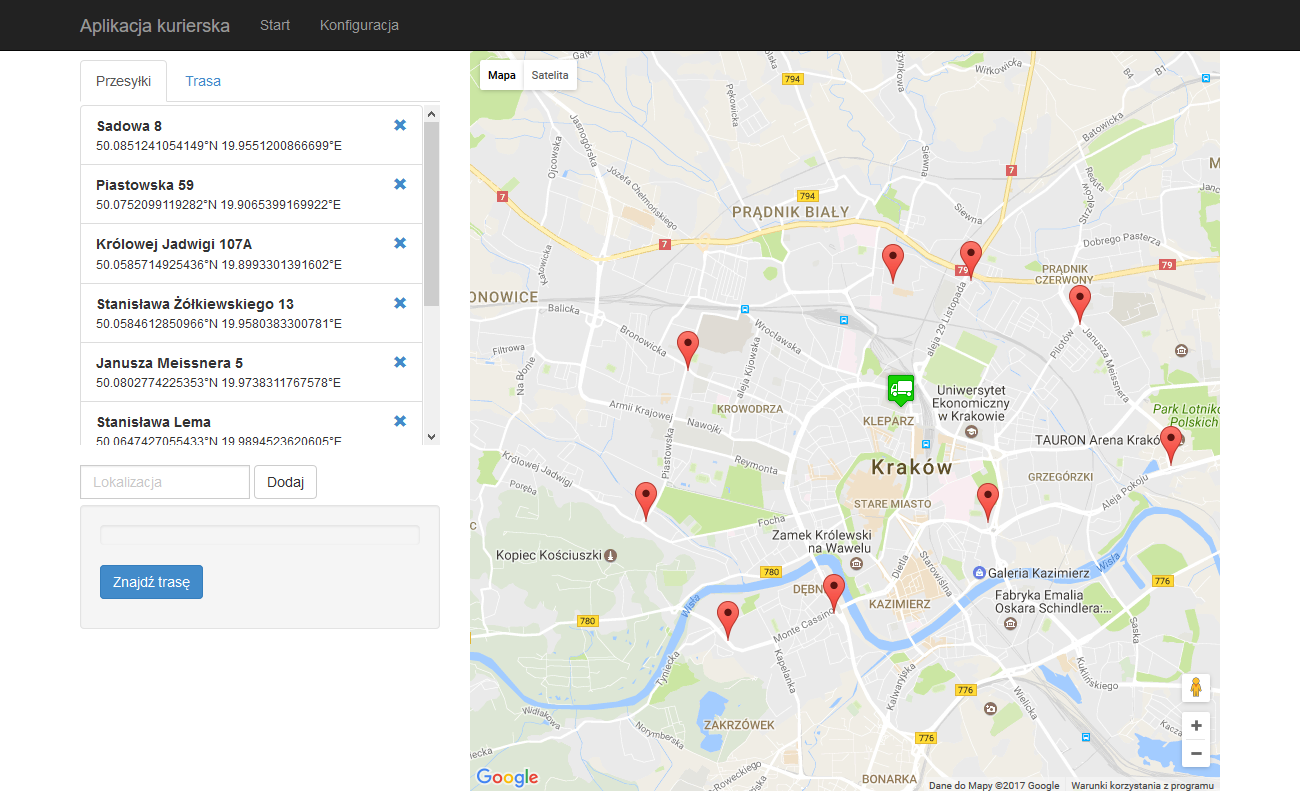
\includegraphics[width=0.7\linewidth]{screen/1_przed_uruchomieniem}
	\caption{Widok aplikacji po dodaniu kilku przesyłek}
	\label{screen:1_przed_uruchomieniem}
\end{figure}

Dodanie przesyłek jest możliwe na dwa sposoby: 
\begin{itemize}
	\item kliknięcie na mapie -- w tym wypadku przybliżony adres zostanie automatycznie znaleziony na podstawie współrzędnych,
	\item wpisanie adresu i naciśnięcie przycisku ,,Dodaj'' -- współrzędne zostaną odnalezione przez wyszukanie adresu.
\end{itemize}

Rezultatem w obu przypadkach jest dodanie przesyłki do listy oraz odpowiedniego punktu na mapie.

Po wprowadzeniu wszystkich punktów, należy nacisnąć przycisk ,,Znajdź trasę''. Uruchamia to proces wyszukiwania trasy na serwerze, a użytkownik widzi w tym czasie animację paska postępu. W przypadku wystąpienia błędu, na przykład z połączeniem, zostanie wyświetlony komunikat z opisem błędu.

Gdy serwer zwróci poprawną odpowiedź (rysunek \ref{screen:2_po_wyszukaniu}), na mapie pokazują się połączenia między punktami trasy. Kolor paska postępu zmienia się na zielony, a poniżej można odczytać łączną długość lub czas potrzebny do przebycia trasy (w zależności od wybranego przez użytkownika sposobu optymalizacji).

\begin{figure}
	\centering
	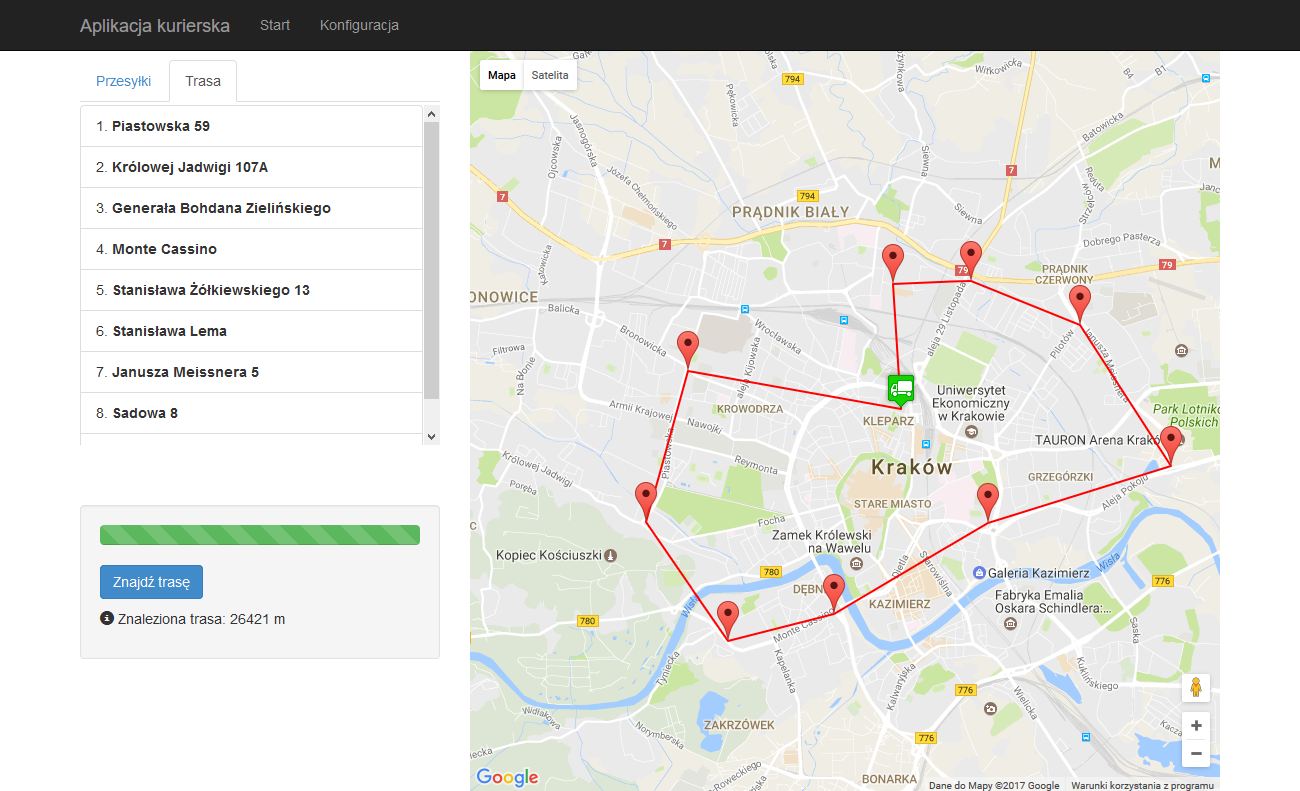
\includegraphics[width=0.7\linewidth]{screen/2_po_wyszukaniu}
	\caption{Mapa z widoczną trasą oraz lista kolejnych celów}
	\label{screen:2_po_wyszukaniu}
\end{figure}

Po wybraniu z menu odnośnika ,,Konfiguracja'' użytkownik ma możliwość zmiany ustawień aplikacji (rysunek \ref{screen:3_konfiguracja}). Okno zostało podzielone na opcje podstawowe, oraz ustawienia silnika przeznaczone dla zaawansowanych użytkowników.

Naciśnięcie przycisku ,,Przywróć domyślne'' resetuje wszystkie ustawienia do stanu początkowego.

Konfiguracja jest zapisywana na dysku serwera w pliku JSON, przez co wartości mogą być odczytane po restarcie serwera.

Do podstawowych opcji należy wybór jednego z trzech rodzajów optymalizacji. Użytkownik ma możliwość wybrania punktu początkowego, czyli siedziby firmy kurierskiej. Wyboru tej lokalizacji dokonuje się poprzez wpisanie adresu lub nazwy miejsca. Aplikacja na bieżąco podpowiada wpisywane adresy.

\begin{figure}
	\centering
	\subcaptionbox{wszystkie dostępne ustawienia\label{screen:3_konfiguracja}}
	{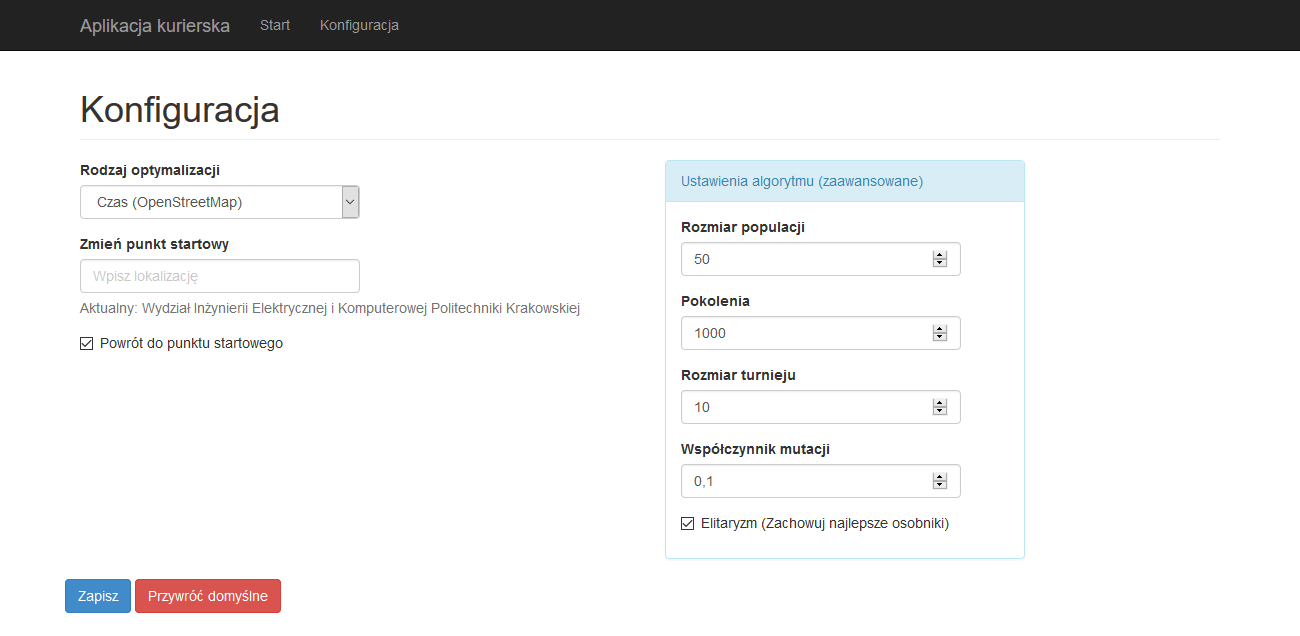
\includegraphics[width=\linewidth]{screen/3_konfiguracja}}
	
	\bigskip
	
	\subcaptionbox{zmiana rodzaju optymalizacji}[0.45\linewidth]
	{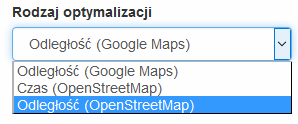
\includegraphics[width=0.4\linewidth]{screen/4a_konfiguracja_cel}}\hfill
	\subcaptionbox{wybór punktu początkowego}[0.45\linewidth]
	{
\includegraphics[width=0.4\linewidth]{screen/4b_konfiguracja_start}}
	
	\caption{Ekran konfiguracji}
\end{figure}

\clearpage

W zaawansowanych ustawieniach można dokonać konfiguracji parametrów algorytmu genetycznego. Pozwala to dostosować aplikację do wymagań konkretnego użytkownika, który może preferować większą dokładność optymalizacji lub jej czas.

Odpowiednie dostrojenie parametrów algorytmu umożliwia znalezienie trasy dla większej liczby przesyłek. Na rysunku \ref{screen:5_wiecej_punktow} aplikacja znalazła optymalną trasę dla 30 punktów.

\begin{figure}[H]
	\centering
	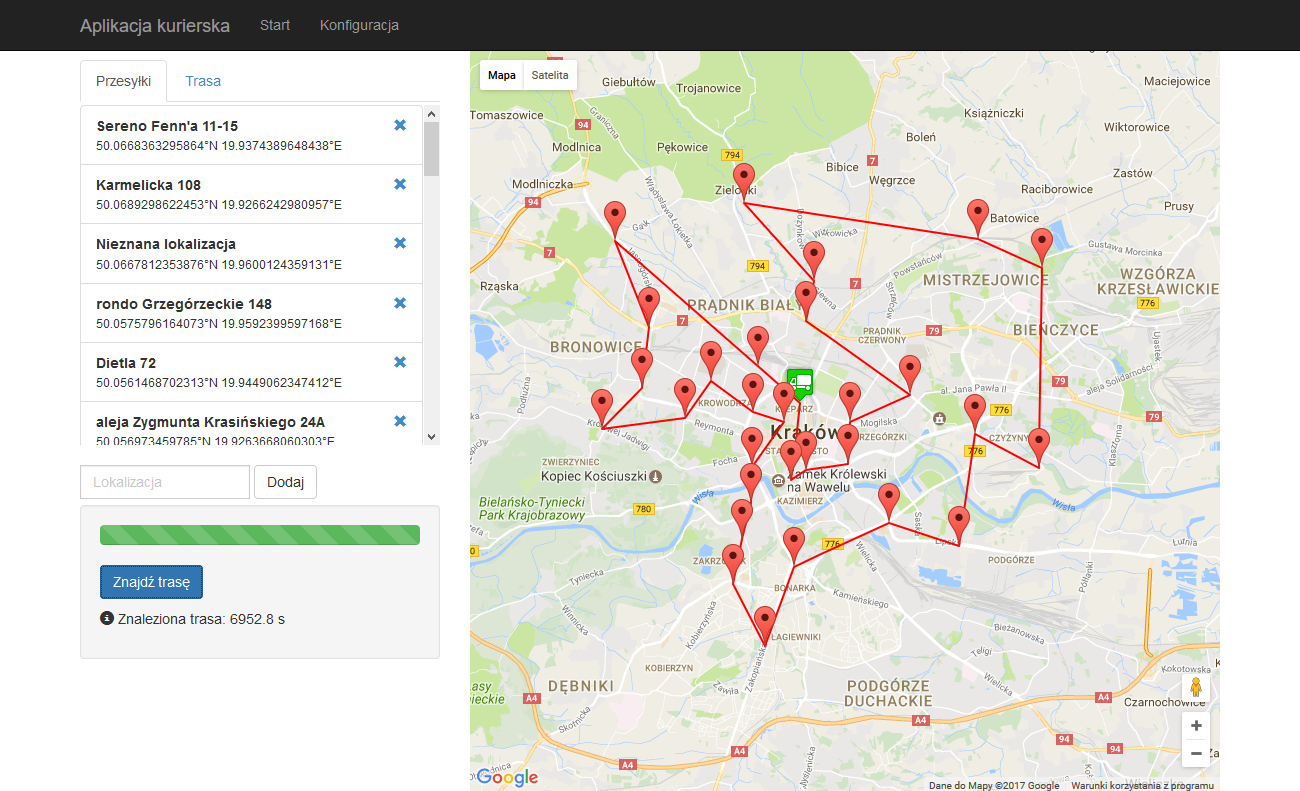
\includegraphics[width=1\linewidth]{screen/5_wiecej_punktow}
	\caption{Znaleziona trasa dla 30 przesyłek}
	\label{screen:5_wiecej_punktow}
\end{figure}

\clearpage